%!TEX TS-program = xelatex
\documentclass{beamer}

\usepackage{HSE-theme/beamerthemeHSE} % Подгружаем тему

%%% Работа с русским языком и шрифтами
\usepackage[english,russian]{babel}   % загружает пакет многоязыковой вёрстки
\usepackage{fontspec}      % подготавливает загрузку шрифтов Open Type, True Type и др.

\defaultfontfeatures{Ligatures={TeX},Renderer=Basic}  % свойства шрифтов по умолчанию
% \setmainfont[Ligatures={TeX,Historic}]{KanjiStrokeOrders.ttf} %  установите шрифты Myriad Pro или (при невозможности) замените здесь на другой шрифт, который есть в системе — например, Arial
\setmainfont[ExternalLocation={./},Ligatures={TeX,Historic}]{MyriadPro-Regular.otf} %  установите шрифты Myriad Pro или (при невозможности) замените здесь на другой шрифт, который есть в системе — например, Arial
\setsansfont[ExternalLocation={./}]{MyriadPro-Regular.otf} %  установите шрифты Myriad Pro или (при невозможности) замените здесь на другой шрифт, который есть в системе — например, Arial
\setmonofont[ExternalLocation={./}]{MyriadPro-Regular.otf}
%\setmonofont{Courier New}

\uselanguage{russian}
\languagepath{russian}
\deftranslation[to=russian]{Theorem}{Теорема}
\deftranslation[to=russian]{Definition}{Определение}
\deftranslation[to=russian]{Definitions}{Определения}
\deftranslation[to=russian]{Corollary}{Следствие}
\deftranslation[to=russian]{Fact}{Факт}
\deftranslation[to=russian]{Example}{Пример}
\deftranslation[to=russian]{Examples}{Примеры}

\usepackage{multicol} 		% Несколько колонок
\graphicspath{{images/}}  	% Папка с картинками

%%% Информация об авторе и выступлении
\title[Курсовая работа]{\scriptsize{%
Факультет компьютерных наук \\%
Департамент программной инженерии \\%
Курсовая работа \\%
}}

\subtitle{Программа скелетная анимация}

\author[Абрамов Артем 151 БПИ]{\scriptsize{%
Выполнил студент группы 151БПИ \\%
Абрамов Артем Михайлович \\%
Научный рюководитель: \\%
доцент департамента программной \\%
инженерии, к.т.н \\%
Ахметсафина Римма Закиевна}}

%\institute[Высшая школа экономики]{Национальный исследовательский университет \\ «Высшая школа экономики» (Москва)}
\date{2016}

\begin{document}	% Начало презентации

\frame[plain]{\titlepage}	% Титульный слайд

%\section{Просто слайд с текстом}
%\subsection{Просто слайд с текстом}

\begin{frame}
\frametitle{Анимация в 3-х мерном пространстве}
	\emph{Что мы хотим записывать в файл} 
	Подходы к анимации: Описание поточечной анимации, опицание, скелетной анимации,Описание анимации с взвешенным воздействием костей на каждую вершину.

\emph{Как именно мы хотим записывать это в файл}
    Возможные форматы для хранения информации: collada, wavefront obj.	
\end{frame}


\begin{frame}
\frametitle{Уже существующие решения}
    Blender, Maya, Cinema4D.
    Дорогие (кроме blender). Сложные в использовании.
    
\end{frame}



\begin{frame}
\frametitle{Цель и задачи работы}
    Реализовать работу алгоритма скелетной анимации.
    \medskip	
	Простая в использовании программа не требующая больших ресурсов для просмотра анимации.
	
	\medskip
    Возможности: Отладка анимации.
\end{frame}


\begin{frame}
\frametitle{Алгоритм скелетная анимация, Стуркура данных}
	Основные определения.
	
	\medskip
	
	Необходимые входные данные. Меш, скелет, весы вершин для каждой кости, набор позицый для скелета в ключевые моменты времени.

\end{frame}


\begin{frame}
\frametitle{Алгоритм скелетная анимация, Созданные вспомогательные структуры}
	Словари, листы, классы и т,д.
\end{frame}



\begin{frame}
\frametitle{Алгоритм скелетная анимация, Блок OpenGL}
	Загрузки в буфер, модификация, материалы, свет, цвет.
\end{frame}




\begin{frame}
\frametitle{Список}
\framesubtitle{Нумерованный список}
	\begin{enumerate} 
		\item Первый пункт:
		\begin{itemize}
			\item подпункт 1;
			\item подпункт 2.
		\end{itemize}
		\item Второй пункт
		\begin{enumerate}
			\item нумерованный подпункт.
		\end{enumerate} 
		\item Третий пункт
	\end{enumerate} 
\end{frame}

\begin{frame}
\frametitle{Список}
\framesubtitle{Маркированный список}
	\begin{itemize}
		\item Первый пункт:
		\begin{itemize}
			\item подпункт 1;
			\item подпункт 2.
		\end{itemize}
		\item Второй пункт
		\begin{enumerate}
			\item нумерованный подпункт.
		\end{enumerate}
		\item Третий пункт
	\end{itemize}
\end{frame}

\begin{frame}
\frametitle{Слайд с двумя колонками текста}
	\begin{multicols}{2}
			\begin{enumerate} 
		\item Первый пункт:
		\begin{itemize}
			\item подпункт 1;
			\item подпункт 2.
		\end{itemize}
		\item Второй пункт
		\begin{enumerate}
			\item нумерованный подпункт.
		\end{enumerate} 
		\item Третий пункт
	\end{enumerate} 
	\columnbreak
	\begin{itemize}
		\item Первый пункт:
		\begin{itemize}
			\item подпункт 1;
			\item подпункт 2.
		\end{itemize}
		\item Второй пункт
		\begin{enumerate}
			\item нумерованный подпункт.
		\end{enumerate}
		\item Третий пункт
	\end{itemize}
	\end{multicols}
\end{frame}

\begin{frame}
\frametitle{Слайд с картинкой}
	\begin{multicols}{2}
		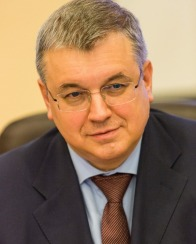
\includegraphics[width=\columnwidth]{kouzminov.png}
		\columnbreak
		До 2014 года в ВШЭ было порядка 40 факультетов и отделений. Весной 2014 года начаты структурные реформы: в университете создаются «большие» факультеты («мегафакультеты»).
		\medskip 

		\textbf{\textit{Ректор}} \\ Высшей школы экономики "--- \alert{Ярослав Иванович Кузьминов}
	\end{multicols}
\end{frame}

\begin{frame}
\frametitle{Блоки}
	\begin{theorem}[Пифагора]
		Если $a$ и $b$ "--- длины катетов прямоугольного треугольника, а~$c$ "--- длина гипотенузы, то $a^2+b^2=c^2$.
	\end{theorem}

	\begin{alertblock}{Блок с красным заголовком}
		Содержимое.
	\end{alertblock}

	\begin{exampleblock}{Блок с зеленым заголовком}
		Содержимое.
	\end{exampleblock}
\end{frame}

\begin{frame}[c]
\begin{center}
\frametitle{\LARGE Спасибо за внимание!}

{\LARGE \inserttitle}

\bigskip

{\insertauthor} 

\bigskip\bigskip

{\insertinstitute}

\bigskip\bigskip

{\large \insertdate}
\end{center}
\end{frame}

\end{document}
